
\section{Nico Ekklesia Sembiring}
\subsection{Apa itu fungsi library matplotlib?}
Library Matplotlib berfungsi untuk membuat visualisasi yang kuat dalam menjelaskan suatu data dalam bentuk diagram dan grafik. 
Contoh grafik yang dapat digambarkan menggunakan Matplotlib adalah :
\begin{itemize}
    \item Grafik Biasa 
    \item Grafik Polar
    \item Chart
    \item Dan yang lainnya
\end{itemize}

\subsection{Jelaskan langkah-langkah membuat sumbu X dan Y di matplotlib}
Langkah langkah membuat Sumbu X dan Y adalah sebagai berikut :
\begin{itemize}
    \item Buat variabel x dan Y
    \item Masukkan nilai dari setiap variabel
    \lstinputlisting[firstline=12, lastline=13]{src/6/Teori/1174096/1174096.py}
    \item Deklarasikan nama dari sumbu x dan y 
    \lstinputlisting[firstline=16, lastline=17]{src/6/Teori/1174096/1174096.py}
\end{itemize}

Setelah dibuat, begini lah hasilnya
\begin{figure}[H]
	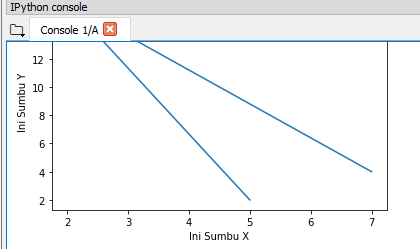
\includegraphics[width=9cm]{figures/6/Teori/1174096/1.png}
	\caption{Hasil membuat sumbu x dan y}
	\centering
\end{figure}

\subsection{Jelaskan bagaimana perbedaan fungsi dan cara pakai untuk berbagai jenis(bar,histogram,scatter,line dll) jenis plot di matplotlib}
Perbedaan fungsi dapat dilihat sebagai berikut :
\begin{itemize}
    \item Graph\linebreak
    Fungsi graph digunakan untuk membuat visualisasi berupa grafik.
    cara pakainya adalah sebagai berikut :
    \lstinputlisting[caption = fungsi untuk membuat graph., firstline=10, lastline=18]{src/6/Teori/1174096/1174096.py}
    hasilnya adalah sebagai berikut:
    \begin{figure}[H]
        \includegraphics[width=9cm]{figures/6/Teori/1174096/3graph.png}
        \caption{Hasil graph}
        \centering
    \end{figure}

    \item Bar\linebreak 
    Fungsi Bar digunakan untuk membuat visualisasi berupa diagram batang yang berhimpit.
    Cara Pakainya adalah sebagai berikut :
    \lstinputlisting[caption = fungsi untuk membuat bar., firstline=22, lastline=32]{src/6/Teori/1174096/1174096.py}
    hasilnya adalah sebagai berikut:
    \begin{figure}[H]
        \includegraphics[width=9cm]{figures/6/Teori/1174096/3bar.png}
        \caption{Hasil bar}
        \centering
    \end{figure}

    \item Histogram\linebreak
    Fungsi Histogram digunakan untuk membuat visualisasi berupa diagram batang yang tidak berhimpit.
    Cara Pakainya adalah sebagai berikut :
    \lstinputlisting[caption = fungsi untuk membuat histogram., firstline=35, lastline=42]{src/6/Teori/1174096/1174096.py}
    hasilnya adalah sebagai berikut:
    \begin{figure}[H]
        \includegraphics[width=9cm]{figures/6/Teori/1174096/3histogram.png}
        \caption{Hasil histogram}
        \centering
    \end{figure}

    \item Scatter\linebreak
    Fungsi Scatter digunakan untuk membuat visualisasi berupa titik titik.
    Cara Pakainya adalah sebagai berikut :
    \lstinputlisting[caption = fungsi untuk membuat scatter., firstline=45, lastline=58]{src/6/Teori/1174096/1174096.py}
    hasilnya adalah sebagai berikut:
    \begin{figure}[H]
        \includegraphics[width=9cm]{figures/6/Teori/1174096/3scatter.png}
        \caption{Hasil scatter}
        \centering
    \end{figure}

    \item Area plot\linebreak
    Fungsi Area plot digunakan untuk membuat visualisasi berupa area.
    Cara Pakainya adalah sebagai berikut :
    \lstinputlisting[caption = fungsi untuk membuat area plot., firstline=61, lastline=80]{src/6/Teori/1174096/1174096.py}
    hasilnya adalah sebagai berikut:
    \begin{figure}[H]
        \includegraphics[width=9cm]{figures/6/Teori/1174096/3areaplot.png}
        \caption{Hasil area plot}
        \centering
    \end{figure}

    \item Pie\linebreak
    Fungsi Pie digunakan untuk membuat visualisasi berupa diagram lingkaran.
    Cara Pakainya adalah sebagai berikut :
    \lstinputlisting[caption = fungsi untuk membuat pie., firstline=83, lastline=104]{src/6/Teori/1174096/1174096.py}
    hasilnya adalah sebagai berikut:
    \begin{figure}[H]
        \includegraphics[width=9cm]{figures/6/Teori/1174096/3pie.png}
        \caption{Hasil pie}
        \centering
    \end{figure}
    
\end{itemize}

\subsection{Jelaskan bagaimana cara menggunakan legend dan label serta kaitannya dengan fungsi tersebut}
Fungsi legend digunakan untuk menjelaskan makna dari objek berupa titik atau garis di dalam diagram.
cara menggunakan legend adalah 
\lstinputlisting[caption = fungsi untuk membuat legend., firstline=24, lastline=28]{src/6/Teori/1174096/1174096.py}
contoh legend :
\begin{figure}[H]
    \includegraphics[width=9cm]{figures/6/Teori/1174096/4legend.png}
    \caption{contoh legend}
    \centering
\end{figure}

\subsection{Jelaskan apa fungsi dari subplot di matplotlib, dan bagaimana cara kerja dari fungsi subplot, sertakan ilustrasi dan gambar sendiri dan apa parameternya jika ingin menggambar plot dengan 9 subplot di dalamnya}
Subplot berfungsi untuk menggabungkan beberapa plot kedalam satu figure
cara kerjanya adalah sebagai berikut
\lstinputlisting[caption = cara kerja subplot., firstline=108, lastline=134]{src/6/Teori/1174096/1174096.py}
Parameter yang digunakan ketika ingin membuat 9 subplot terdiri dari (331) sampai (339). karena posisi subplot dilihat dengan melihat tinggi,lebar,urutan
hasil dari subplot adalah
\begin{figure}[H]
    \includegraphics[width=9cm]{figures/6/Teori/1174096/5subplot.png}
    \caption{hasil subplot}
    \centering
\end{figure}

\subsection{Sebutkan semua parameter color yang bisa digunakan}
Parameter color yang bisa digunakan antara lain RGB dan CMYK
\begin{itemize}
    \item C (Cyan) adalah biru muda
    \item M (Magenta) adalah merah muda
    \item Y (Yellow) adalah kuning
    \item K (Key) adalah hitam
    \item R (Red) adalah merah
    \item G (Green) adalah Hijau
    \item B (Blue) adalah Biru
    
\end{itemize}

\subsection{Jelaskan bagaimana cara kerja dari fungsi hist, sertakan ilustrasi dan gambar sendiri}
cara kerja dari fungsi histogram adalah sebagai berikut :
\lstinputlisting[caption = cara kerja histogram., firstline=137, lastline=144]{src/6/Teori/1174096/1174096.py}
hasilnya adalah
\begin{figure}[H]
    \includegraphics[width=9cm]{figures/6/Teori/1174096/7his.png}
    \caption{histogram}
    \centering
\end{figure}

\subsection{Jelaskan lebih mendalam tentang parameter dari fungsi pie diantaranya labels, colors, startangle, shadow, explode, autopct}
\begin{itemize}
    \item Labels = berfungsi untuk menampilkan tulisan pada diagram pie
    \item Colors = berfungsi untuk menentukan warna pada tiap bagian pada diagram pie
    \item Startangle = berfungsi untuk menentukan sudut pertama pada diagram pie
    \item Shadow = berfungsi untuk menampilkan efek timbul pada diagram pie
    \item Explode = berfungsi untuk menunjukkan jarak pisah dari diagram pie.
    \item Autopct = berfungsi umtuk menampilkan jumlah angka dibelakang koma pada bilangan pecahan
\end{itemize}

\subsection{Pengecekan Plagiarisme Teori}
\begin{figure}[H]
	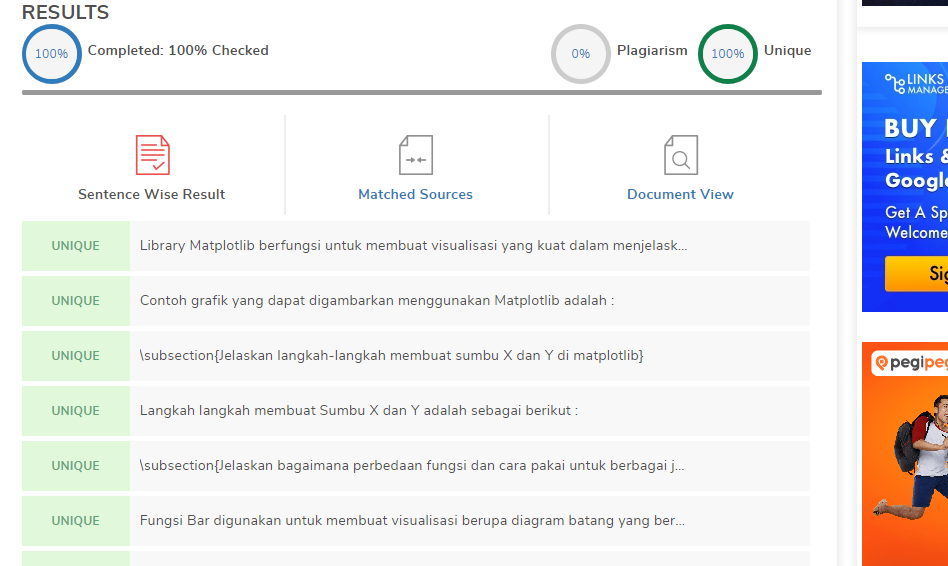
\includegraphics[width=9cm]{figures/6/Teori/1174096/Plagiat.png}
	\centering
\end{figure}

\section{Muhammad Dzihan Al-Banna}
\subsection{Soal 1}
Libarary matplotlib berfungsi untuk menampilkan data grafik yang mudah dibuat dan ditampilkan dengan cara sederhana saja di python yaitu hanya dengan mendefinisikan tabel x dan y kemudian mengisi variabelnya dengan data. Matplotlib sangat berguna untuk data science.
\subsection{Soal 2}
Membuat sumbu x dan y di matplotlib cukup mudah yaitu hanya dengan mengimport matplotlib terlebih dahulu, mendefinisikan fungsi plot dan membuat variable plot dan isi variable x dan y tersebut dengan data. Variable yang diisi pertama adalah sumbu x dan yang kedua adalah sumbu y.

\lstinputlisting[firstline=13, lastline=19]{src/6/Teori/1174095/T1174095_plt.py}
\subsection{Soal 3}
\begin{itemize}
\item Pada penggunaan bar di awal pembuatan fungsi ditambahkan plt.bar  yang pertama kemudian isi datanya, begitu juga yang kedua melakukan hal yang sama.
\lstinputlisting[firstline=22, lastline=32]{src/6/Teori/1174095/T1174095_plt.py}
\item dalam penggunaan histogram juga dilakukan coding seperti diatas pada bar tetapi menggunakan plt.hist
\item jika mau menggunakan fungsi scatter maka diganti dengan plt.scatter, jika menggunakan scatter maka grafiknya akan ditandai dengan titik.
\lstinputlisting[firstline=35, lastline=48]{src/6/Teori/1174095/T1174095_plt.py}
\end{itemize}
\subsection{Soal 4}
Membuat legend pertama-tama gunakan dulu style.use('ggplot') setelah itu buat plt.xlabel dan plt.ylabel sebagai penanda bahwa itu sumbu x dan y. setelah itu tambahkan plt.legend.
\lstinputlisting[firstline=51, lastline=66]{src/6/Teori/1174095/T1174095_plt.py}
\subsection{Soal 5}
\begin{figure}[h]
\centering
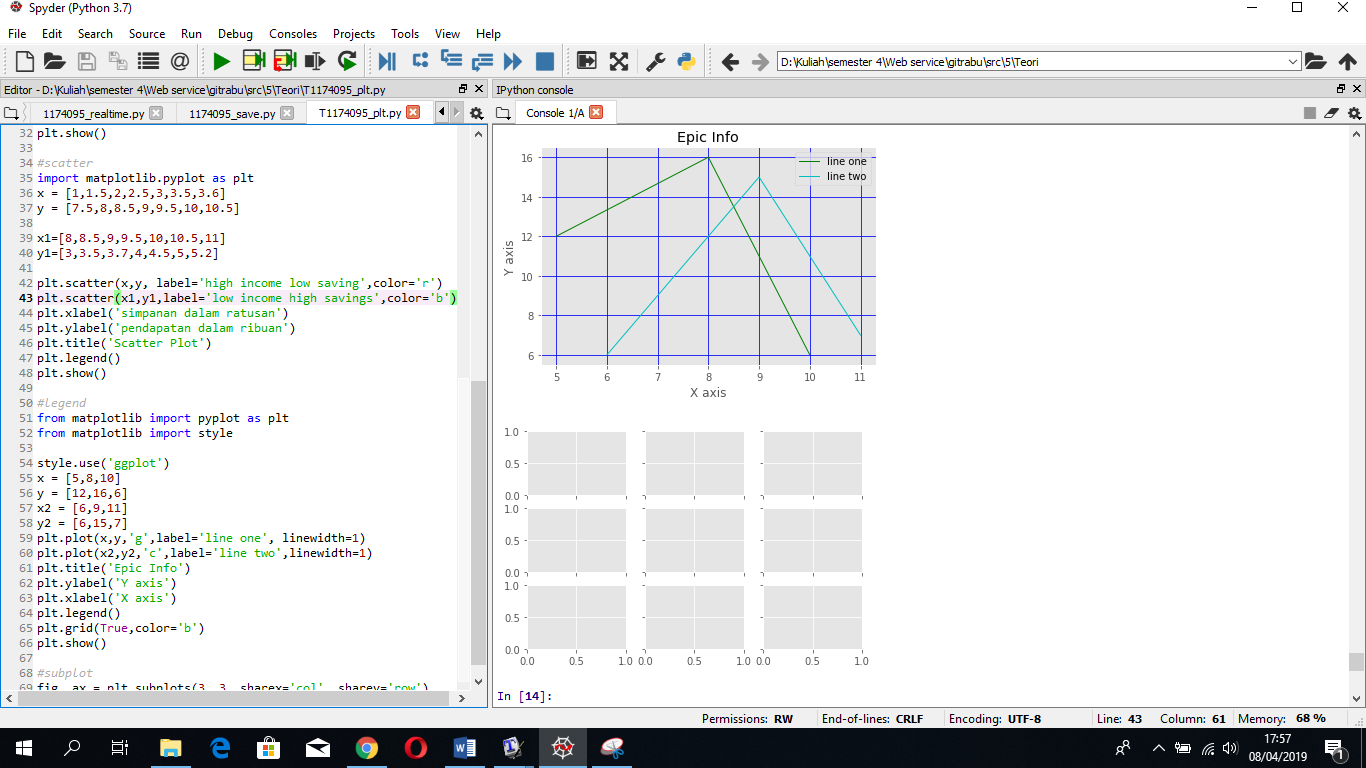
\includegraphics[width=20cm]{figures/6/Teori/1174095/ssub.png}
\caption{Sub Plot}
\label{Dzihan}
\end{figure}
sublot berfungsi untuk menampilkan banyak plot dalam satu grafik.
\begin{itemize}
\item buat fungsi subplot
\item isi parameternya
\item definisikan colomn dan rownya.
\item atur range yang ingin ditampilkan
\item Jika ingin membuat 9 sublot maka atur rangenya menjadi 3,3 agar rownya terisi 3 dan coloumnnya 3.
\end{itemize}
\subsection{Soal 6}
Parameter color yang bisa digunakan dalam library maplotlib adalah RGB dan CMYK.
\subsection{Soal 7}
Cara untuk menampilkan hist adalah dengan menggunakan plt.hist. caranya adalah sebagai berikut :
\lstinputlisting[firstline=72, lastline=79]{src/6/Teori/1174095/T1174095_plt.py}
\subsection{Soal 8}
\begin{enumerate}
\item label digunakan untuk menandai bagian tertentu seperti sumbu x atau sumbu y
\item colors digunakan untuk memberikan warna di bagian table pada data grafik
\item startangle digunakan untuk memutar balikan table dengan arah kebalikannya.
\item shadow digunakan untuk memberikan bayangan pada data agar terlihat seperti 3D.
\item explode digunakan untuk menonjolkan data dari grafik tertentu agar terlihat lebih mencolok.
\item autocpt digunakan untuk memberi persen pada bagian paychart yang dibuat.
\end{enumerate}

\section{Choirul Anam}
\subsection{Apa itu fungsi library matplotlib?}
Library Matplotlib memiliki fungsi untuk visualisasi yang menampilkan suatu data dalam bentuk diagram dan grafik. 
Berikut contoh grafik-grafik yang dapat digambarkan menggunakan Library Matplotlib :
\begin{itemize}
    \item Grafik Biasa 
    \item Grafik Polar
    \item Chart
    \item Dan yang lainnya
\end{itemize}

\subsection{Jelaskan langkah-langkah membuat sumbu X dan Y di matplotlib}
Langkah langkah membuat Sumbu X dan Y adalah sebagai berikut :
\begin{itemize}
    \item Buatlah variabel x dan Y
    \item input nilai pada variable
    \lstinputlisting[firstline=12, lastline=13]{src/6/Teori/1174004/1174004.py}
    \item Deklarasikan nama dari sumbu x dan y 
    \lstinputlisting[firstline=16, lastline=17]{src/6/Teori/1174004/1174004.py}
\end{itemize}

Berikut Hasilnya
\begin{figure}[H]
	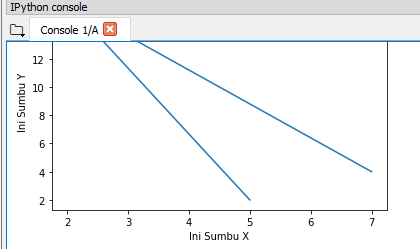
\includegraphics[width=9cm]{figures/6/Teori/1174096/1.png}
	\caption{Hasil membuat sumbu x dan y}
	\centering
\end{figure}

\subsection{Jelaskan bagaimana perbedaan fungsi dan cara pakai untuk berbagai jenis(bar,histogram,scatter,line dll) jenis plot di matplotlib}
Perbedaan fungsi dapat dilihat sebagai berikut :
\begin{itemize}
    \item Graph
    \linebreak
    Fungsi graph digunakan untuk membuat visualisasi berupa grafik.
    cara pakainya adalah sebagai berikut :
    \lstinputlisting[caption = fungsi untuk membuat graph., firstline=10, lastline=18]{src/6/Teori/1174004/1174004.py}
    hasilnya adalah sebagai berikut:
    \begin{figure}[H]
        \includegraphics[width=9cm]{figures/6/Teori/1174004/3graph.png}
        \caption{Hasil graph}
        \centering
    \end{figure}

    \item Bar
    \linebreak 
    Fungsi Bar digunakan untuk membuat visualisasi berupa diagram batang yang berhimpit.
    Cara Pakainya adalah sebagai berikut :
    \lstinputlisting[caption = fungsi untuk membuat bar., firstline=22, lastline=32]{src/6/Teori/1174004/1174004.py}
    hasilnya adalah sebagai berikut:
    \begin{figure}[H]
        \includegraphics[width=9cm]{figures/6/Teori/1174004/3bar.png}
        \caption{Hasil bar}
        \centering
    \end{figure}

    \item Histogram
    \linebreak
    Fungsi Histogram digunakan untuk membuat visualisasi berupa diagram batang yang tidak berhimpit.
    Cara Pakainya adalah sebagai berikut :
    \lstinputlisting[caption = fungsi untuk membuat histogram., firstline=35, lastline=42]{src/6/Teori/1174004/1174004.py}
    hasilnya adalah sebagai berikut:
    \begin{figure}[H]
        \includegraphics[width=9cm]{figures/6/Teori/1174004/3histogram.png}
        \caption{Hasil histogram}
        \centering
    \end{figure}

    \item Scatter
    \linebreak
    Fungsi Scatter digunakan untuk membuat visualisasi berupa titik titik.
    Cara Pakainya adalah sebagai berikut :
    \lstinputlisting[caption = fungsi untuk membuat scatter., firstline=45, lastline=58]{src/6/Teori/1174004/1174004.py}
    hasilnya adalah sebagai berikut:
    \begin{figure}[H]
        \includegraphics[width=9cm]{figures/6/Teori/1174004/3scatter.png}
        \caption{Hasil scatter}
        \centering
    \end{figure}

    \item Area plot
    \linebreak
    Fungsi Area plot digunakan untuk membuat visualisasi berupa area.
    Cara Pakainya adalah sebagai berikut :
    \lstinputlisting[caption = fungsi untuk membuat area plot., firstline=61, lastline=80]{src/6/Teori/1174004/1174004.py}
    hasilnya adalah sebagai berikut:
    \begin{figure}[H]
        \includegraphics[width=9cm]{figures/6/Teori/1174004/3areaplot.png}
        \caption{Hasil area plot}
        \centering
    \end{figure}

    \item Pie
    \linebreak
    Fungsi Pie digunakan untuk membuat visualisasi berupa diagram lingkaran.
    Cara Pakainya adalah sebagai berikut :
    \lstinputlisting[caption = fungsi untuk membuat pie., firstline=83, lastline=104]{src/6/Teori/1174004/1174004.py}
    hasilnya adalah sebagai berikut:
    \begin{figure}[H]
        \includegraphics[width=9cm]{figures/6/Teori/1174004/3pie.png}
        \caption{Hasil pie}
        \centering
    \end{figure}
    
\end{itemize}

\subsection{Jelaskan bagaimana cara menggunakan legend dan label serta kaitannya dengan fungsi tersebut}
Fungsi legend digunakan dalam menjelaskan makna dari objek berupa titik atau garis di dalam diagram.
cara menggunakan legend adalah 
\lstinputlisting[caption = fungsi untuk membuat legend., firstline=24, lastline=28]{src/6/Teori/1174004/1174004.py}
contoh legend :
\begin{figure}[H]
    \includegraphics[width=9cm]{figures/6/Teori/1174004/4legend.png}
    \caption{contoh legend}
    \centering
\end{figure}

\subsection{Jelaskan apa fungsi dari subplot di matplotlib, dan bagaimana cara kerja dari fungsi subplot, sertakan ilustrasi dan gambar sendiri dan apa parameternya jika ingin menggambar plot dengan 9 subplot di dalamnya}
Subplot berfungsi untuk menggabungkan beberapa plot kedalam satu figure.
cara kerjanya adalah sebagai berikut
\lstinputlisting[caption = cara kerja subplot., firstline=108, lastline=134]{src/6/Teori/1174004/1174004.py}
Parameter yang digunakan ketika ingin membuat 9 subplot terdiri dari (331) sampai (339). karena posisi subplot dilihat dengan melihat tinggi,lebar,urutan
hasil dari subplot adalah
\begin{figure}[H]
    \includegraphics[width=9cm]{figures/6/Teori/1174004/5subplot.png}
    \caption{hasil subplot}
    \centering
\end{figure}

\subsection{Sebutkan semua parameter color yang bisa digunakan}
Parameter color yang bisa digunakan antara lain RGB dan CMYK
\begin{itemize}
    \item C (Cyan) adalah biru muda
    \item M (Magenta) adalah merah muda
    \item Y (Yellow) adalah kuning
    \item K (Key) adalah hitam
    \item R (Red) adalah merah
    \item G (Green) adalah Hijau
    \item B (Blue) adalah Biru
\end{itemize}

\subsection{Jelaskan bagaimana cara kerja dari fungsi hist, sertakan ilustrasi dan gambar sendiri}
cara kerja dari fungsi histogram adalah sebagai berikut :
\lstinputlisting[caption = cara kerja histogram., firstline=137, lastline=144]{src/6/Teori/1174004/1174004.py}
hasilnya adalah
\begin{figure}[H]
    \includegraphics[width=9cm]{figures/6/Teori/1174004/7his.png}
    \caption{histogram}
    \centering
\end{figure}

\subsection{Jelaskan lebih mendalam tentang parameter dari fungsi pie diantaranya labels, colors, startangle, shadow, explode, autopct}
\begin{itemize}
    \item Labels = berfungsi untuk menampilkan tulisan pada diagram pie
    \item Colors = berfungsi untuk menentukan warna pada tiap bagian pada diagram pie
    \item Startangle = berfungsi untuk menentukan sudut pertama pada diagram pie
    \item Shadow = berfungsi untuk menampilkan efek timbul pada diagram pie
    \item Explode = berfungsi untuk menunjukkan jarak pisah dari diagram pie.
    \item Autopct = berfungsi umtuk menampilkan jumlah angka dibelakang koma pada bilangan pecahan
\end{itemize}

\subsection{Pengecekan Plagiarisme Teori}
\begin{figure}[H]
	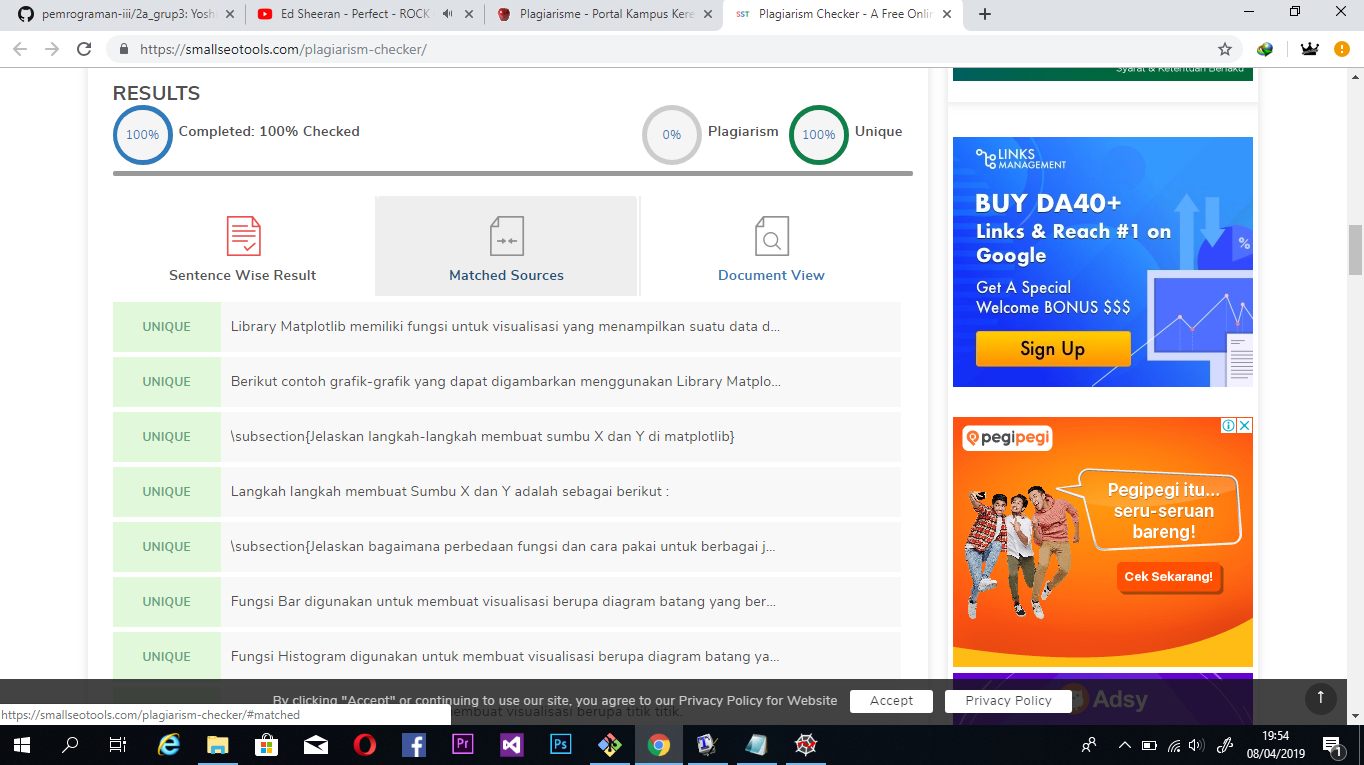
\includegraphics[width=9cm]{figures/6/Teori/1174004/Plagiat.png}
	\centering
\end{figure}

\section{Habib Abdul Rasyid}
\subsection{ Apa itu fungsi library matplotlib}
Library matplotlib.pyplot adalah kumpulan fungsi atau gaya perintah yang membuat matplotlib berfungsi seperti MATLAB. Setiap fungsi plot membuat beberapa perubahan pada gambar: misalnya., Membuat gambar, membuat area plot pada gambar, plot beberapa garis di area plot, menghias plot dengan label, dll. Berikut adalah contoh import library mtplotlib.pyplot :

\lstinputlisting[firstline=8, lastline=8]{src/6/Teori/1174002/1174002.py}

\subsection{Jelaskan langkah-langkah membuat sumbu X dan Y di matplotlib}
Langkah untuk membuat Sumbu X dan Y :
\begin{enumerate}
	\item Pastikan matplotlib.pyplot nya sudah di import kedalam file py nya.
	\item Untuk mempermudah memahaminya buatlah Variable X dan Y yang berisi angka Kordinat dari masing masing Sumbu.
	\item Kemudian Variable dipanggil ke dalam perintah plt.plot, contohnya plt.plot(x,y)
	\item Untuk menampilkan grafik nya maka buat perintah plt.show()
	\item Berikut adalah contoh Kodingan dan Hasilnya
\end{enumerate}
\lstinputlisting[firstline=7, lastline=14]{src/6/Teori/1174002/1174002.py}

\begin{figure}[h]
\centering
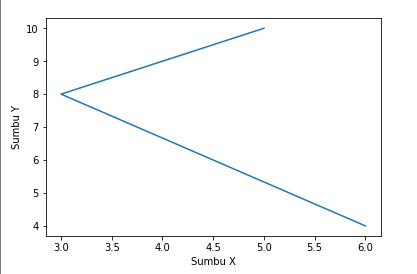
\includegraphics[scale=0.7]{figures/6/Teori/1174002/no2.png}
\caption{Contoh Hasil pembuatan Sumbu X dan Y}
\label{fig:contoh}
\end{figure}

\subsection{Jelaskan bagaimana perbedaan fungsi dan cara pakai untuk berbagai jenis(bar,histogram,scatter,line dll) jenis plot di matplotlib}
\begin{itemize}
	\item Bar\newline
	Bar ini berfungsi menampilkan grafik Bar secara vertikal biasanya digunakan untuk traffic penjualan.\newline
	Cara menggunakan bar cukup ganti plt.plot menjadi plt.bar seperti pada contoh berikut :

	\lstinputlisting[firstline=18, lastline=26]{src/6/Teori/1174002/1174002.py}

\begin{figure}[h]
\centering
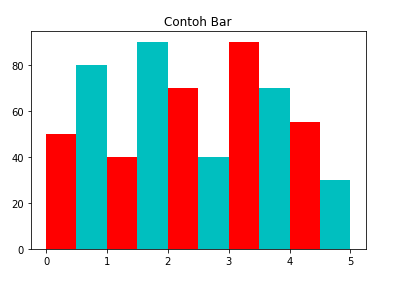
\includegraphics[scale=0.3]{figures/6/Teori/1174002/no3bar.png}
\caption{Contoh Hasil Bar}
\label{fig:contoh}
\end{figure}
\end{itemize}

\begin{itemize}	
	\item Histogram\newline
	Histogram dapat menampilkan grafik sesuai kebutuhan contohnya menampilkan grafik bar, akan tetapi histogram ini
	tidak mengacu pada sumbu X dan Y, artinya sumbu X dan Y jumlah datanya tidak harus sama. biasanya digunakan
	untuk menghitung jumlah populasi.\newline
	Cara menggunakannya yaitu dengan perintah plt.hist, Berikut adalah Contohnya :

	\lstinputlisting[firstline=29, lastline=35]{src/6/Teori/1174002/1174002.py}

\begin{figure}[h]
\centering
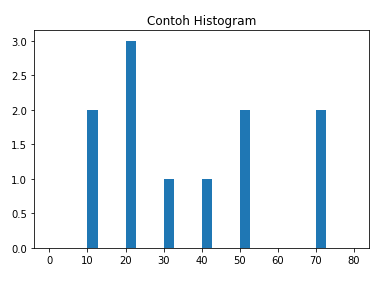
\includegraphics[scale=0.9]{figures/6/Teori/1174002/no3histogram.png}
\caption{Contoh Hasil Histogram}
\label{fig:contoh}
\end{figure}
\end{itemize}

\begin{itemize}
	\item Line\newline
	Line merupakan Plot grafik yang hanya menggambarkan sebuah garis sesuai kordinat yang kita atur.
	Cara menggunakannya Cukup ketik perintah plt.plot

	\lstinputlisting[firstline=7, lastline=14]{src/6/Teori/1174002/1174002.py}

\begin{figure}[h]
\centering
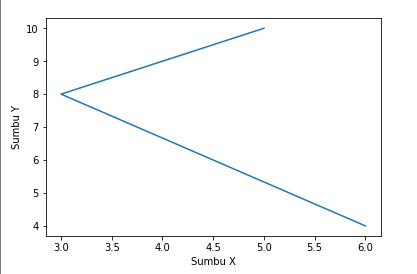
\includegraphics[scale=0.6]{figures/6/Teori/1174002/no2.png}
\caption{Contoh Plot Line}
\label{fig:contoh}
\end{figure}
\end{itemize}

\begin{itemize}	
	\item Scatter\newline
	Scatter merupakan grafik yang didalamnya dapat berisi 2 data dalam 1 plot.\newline
	Cara menggunakan Scatter menggunakan perintah plt.scatter, Berikut adalah contohnya :

	\lstinputlisting[firstline=37, lastline=52]{src/6/Teori/1174002/1174002.py}

\begin{figure}[h]
\centering
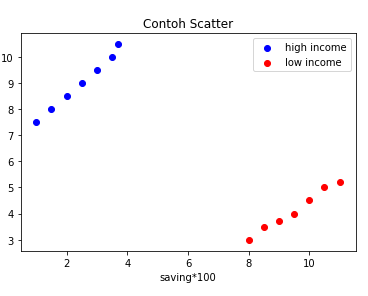
\includegraphics[scale=0.5]{figures/6/Teori/1174002/no3scatter.png}
\caption{Contoh Hasil Scatter}
\label{fig:contoh}
\end{figure}
\end{itemize}

\begin{itemize}
	\item Pie\newline
	Chart Pie merupakan grafik yang membentuk sperti kue Pie, dimana cara penggunaannya adalah dengan perintah
	plt.pie seperti pada contoh berikut :
	
	\lstinputlisting[firstline=54, lastline=75]{src/6/Teori/1174002/1174002.py}

\begin{figure}[h]
\centering
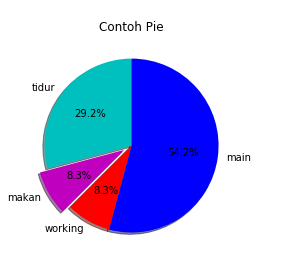
\includegraphics[scale=0.6]{figures/6/Teori/1174002/no3pie.png}
\caption{Contoh Hasil Pie}
\label{fig:contoh Pie}
\end{figure}


\end{itemize}

\subsection{Jelaskan bagaimana cara menggunakan legend dan label serta kaitannya dengan fungsi tersebut}
Legend digunakan untuk menampilkan keterangan tanda pada grafik, label digunakan untuk penamaan tanda tersebut.
berikut adalah syntax untuk menampilkan legend dan penamaan label.

\lstinputlisting[firstline=46, lastline=52]{src/6/Teori/1174002/1174002.py}

\begin{figure}[h]
\centering
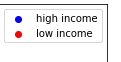
\includegraphics[scale=1]{figures/6/Teori/1174002/no4legend.png}
\caption{Contoh Hasil Legend dan Label}
\label{fig:contoh Legend}
\end{figure}

\subsection{Jelaskan apa fungsi dari subplot di matplotlib, dan bagaimana cara kerja dari fungsi subplot, sertakan ilustrasi dan gambar sendiri dan apa parameternya jika ingin menggambar plot dengan 9 subplot di dalamnya}
Subplot Merupakan Plot didalam dimana Plot ini biasanya berukuran kecil sehingga dapat memuat 2 atau lebih plot dalam 1 paket Plot.\newline
Jika ingin membuat 9 subplot maka buat perintah plt.subplot dengan parameter angka awal 3 angka kedua 3 dan angka ketiga 1, artinya angka awal adalah batas jumlah plot secara vertical, angka kedua adalah batas plot secara horizontal, dan angka ketiga adalah urutan plot nya.
Berikut ini adalah Ilustrasi subplot.

\lstinputlisting[firstline=77, lastline=110]{src/6/Teori/1174002/1174002.py}

\begin{figure}[h]
\centering
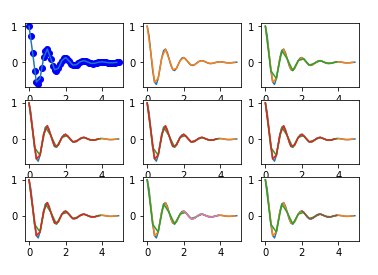
\includegraphics[scale=0.7]{figures/6/Teori/1174002/subplot.png}
\caption{Contoh 9 Subplot}
\label{fig:contoh subplot}
\end{figure}

\subsection{ Sebutkan semua parameter color yang bisa digunakan (contoh: m,c,r,k,... dkk)}
\begin{enumerate}
	\item Parameter yang dapat digunakan adalah CMYK :
\end{enumerate}
 
\begin{itemize}
	\item C = Biru Muda
	\item M = Ungu
	\item Y = Kuning
	\item K = Hitam
\end{itemize}

\begin{enumerate}
	\item Parameter yang kedua adalah RGB, selain menggunakan RGB nya kita juga dapat menggunakan kode warna dari RGB.
\end{enumerate}

\begin{itemize}
	\item R = merah
	\item G = hijau
	\item B = blue
\end{itemize}

\subsection{Jelaskan bagaimana cara kerja dari fungsi hist, sertakan ilustrasi dan gambar sendiri}
Fungsi hist digunakan untuk memanggil Histogram, diamana Histogram dapat menampilkan grafik sesuai kebutuhan contohnya menampilkan grafik bar, akan tetapi histogram ini tidak mengacu pada sumbu X dan Y, artinya sumbu X dan Y jumlah datanya tidak harus sama. biasanya digunakan untuk menghitung jumlah populasi.\newline
	Cara menggunakannya yaitu dengan perintah plt.hist, Berikut adalah Contohnya :

	\lstinputlisting[firstline=29, lastline=35]{src/6/Teori/1174002/1174002.py}

\begin{figure}[h]
\centering
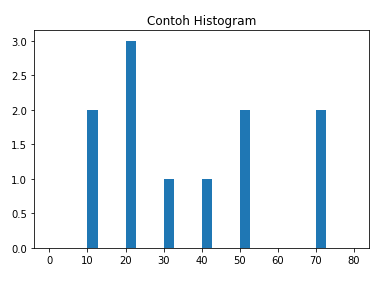
\includegraphics[scale=0.7]{figures/6/Teori/1174002/no3histogram.png}
\caption{Contoh Hasil Histogram}
\label{fig:contoh}
\end{figure}

\subsection{Jelaskan lebih mendalam tentang parameter dari fungsi pie diantaranya labels, colors, startangle, shadow, explode, autopct}
\begin{itemize}
	\item Labels\newline
	Labels pada Pie adalah untuk menambahkan Keterangan pada Pie diamana labels ini biasanya adalah Variabel yang dialamnya berisi data array
	\item Colors\newline
	Colors pada pie adalah untuk mendefinisikan warna pada setiap potongannya.
	\item Startangle\newline
	Startangle adalah untuk mengatur perputaran potongan Pie nya dimulai dari berapa derajat.
	\item Shadow\newline
	Shadow adalah untuk mengatur ketebalan bayangan pada Pie.
	\item Explode\newline
	Explode ini untuk Mengatur Jarak Pie yang dipotong keluar.
	\item Autopct\newline
	Autopct ini adalah untuk perhitungan persen yang mana kita dapat mengatur berapa angka di belakang koma nya. 
\end{itemize}

\subsection{Plagiarisme}
\begin{figure}[h]
\centering
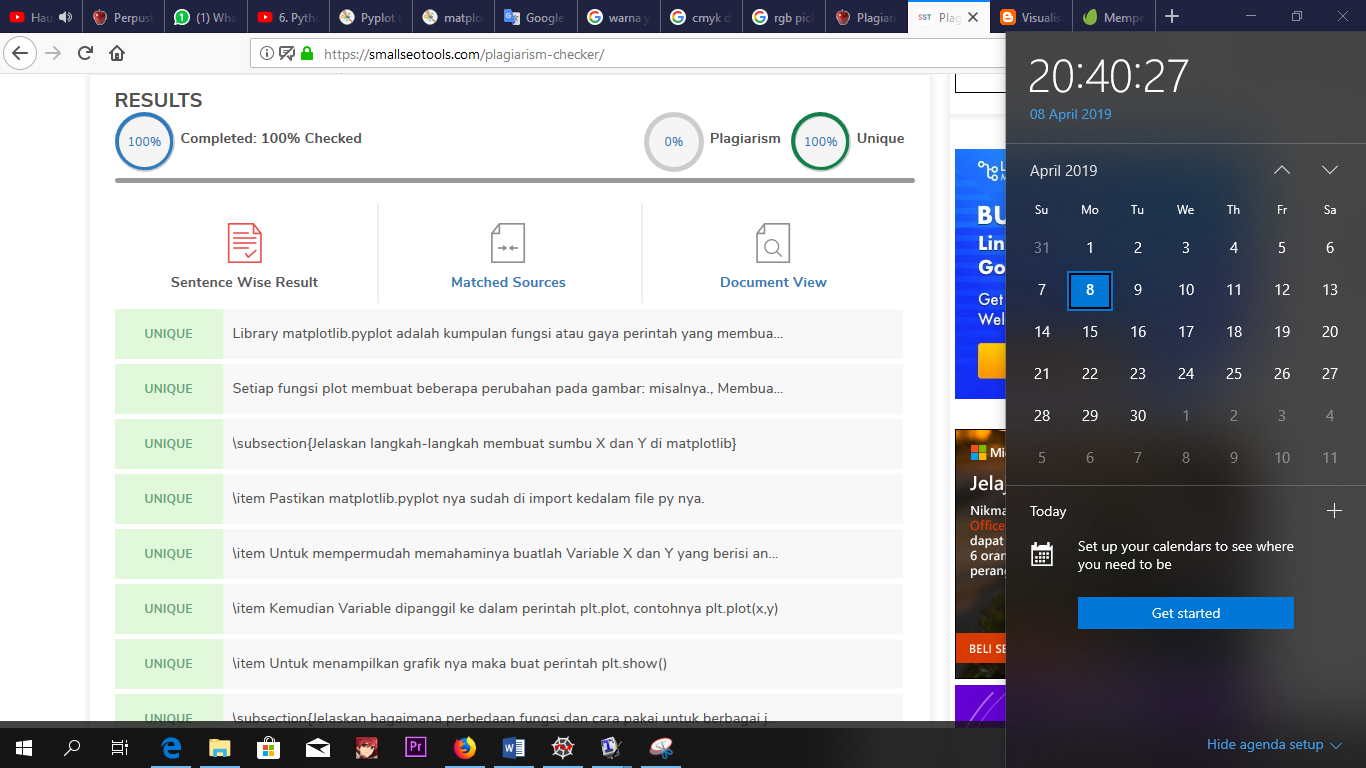
\includegraphics[scale=0.2]{figures/6/Teori/1174002/8april.png}
\caption{Plagiarisme}
\label{fig:plagiat}
\end{figure}


\section{Dezha Aidil Martha}
\subsection{ Apa itu fungsi library matplotlib}
Library matplotlib.pyplot merupakan kumpulan fungsi atau perintah yang membuat matplotlib berfungsi seperti MATLAB. Setiap fungsi plot membuat beberapa perubahan pada gambar: misalnya., Membuat gambar, membuat area plot pada gambar, plot beberapa garis di area plot, menghias plot dengan label, dll. Berikut adalah contoh import library mtplotlib.pyplot :

\lstinputlisting[firstline=8, lastline=8]{src/6/Teori/1174025/1174025.py}

\subsection{Jelaskan langkah-langkah membuat sumbu X dan Y di matplotlib}
Langkah untuk membuat Sumbu X dan Y :
\begin{enumerate}
	\item Pastikan matplotlib.pyplot nya sudah di import kedalam file py nya.
	\item Untuk mempermudah memahaminya buatlah Variable X dan Y yang berisi angka Kordinat dari masing masing Sumbu.
	\item Kemudian Variable dipanggil ke dalam perintah plt.plot, contohnya plt.plot(x,y)
	\item Untuk menampilkan grafik nya maka buat perintah plt.show()
	\item Berikut adalah contoh Kodingan dan Hasilnya
\end{enumerate}
\lstinputlisting[firstline=7, lastline=14]{src/6/Teori/1174025/1174025.py}

\begin{figure}[h]
\centering
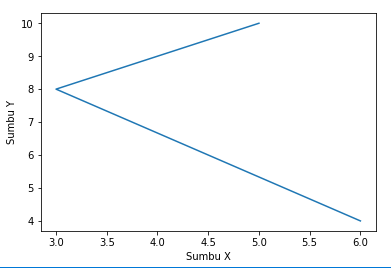
\includegraphics[scale=0.7]{figures/6/Teori/1174025/no2.png}
\caption{Contoh Hasil pembuatan Sumbu X dan Y}
\label{fig:contoh}
\end{figure}

\subsection{Jelaskan bagaimana perbedaan fungsi dan cara pakai untuk berbagai jenis(bar,histogram,scatter,line dll) jenis plot di matplotlib}
\begin{itemize}
	\item Bar\newline
	Bar ini berfungsi menampilkan grafik Bar secara vertikal biasanya digunakan untuk traffic penjualan.\newline
	Cara menggunakan bar cukup ganti plt.plot menjadi plt.bar seperti pada contoh berikut :

	\lstinputlisting[firstline=18, lastline=26]{src/6/Teori/1174025/1174025.py}

\begin{figure}[h]
\centering
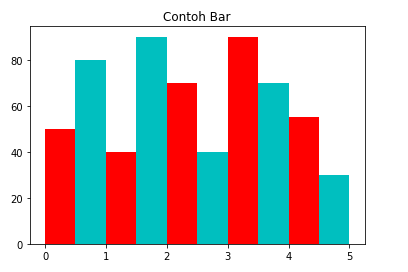
\includegraphics[scale=0.3]{figures/6/Teori/1174025/no3b.png}
\caption{Contoh Hasil Bar}
\label{fig:contoh}
\end{figure}
\end{itemize}

\begin{itemize}	
	\item Histogram\newline
	Histogram dapat menampilkan grafik sesuai kebutuhan contohnya menampilkan grafik bar, akan tetapi histogram ini
	tidak mengacu pada sumbu X dan Y, artinya sumbu X dan Y jumlah datanya tidak harus sama. biasanya digunakan
	untuk menghitung jumlah populasi.\newline
	Cara menggunakannya yaitu dengan perintah plt.hist, Berikut adalah Contohnya :

	\lstinputlisting[firstline=29, lastline=35]{src/6/Teori/1174025/1174025.py}

\begin{figure}[h]
\centering
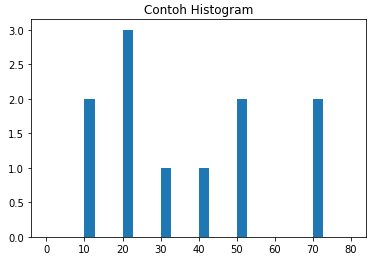
\includegraphics[scale=0.9]{figures/6/Teori/1174025/no3h.png}
\caption{Contoh Hasil Histogram}
\label{fig:contoh}
\end{figure}
\end{itemize}

\begin{itemize}
	\item Line\newline
	Line merupakan Plot grafik yang hanya menggambarkan sebuah garis sesuai kordinat yang kita atur.
	Cara menggunakannya Cukup ketik perintah plt.plot

	\lstinputlisting[firstline=7, lastline=14]{src/6/Teori/1174025/1174025.py}

\begin{figure}[h]
\centering
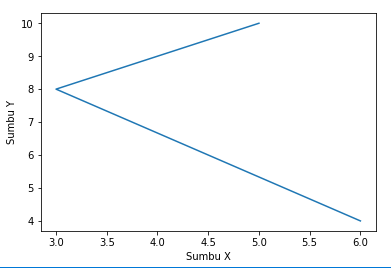
\includegraphics[scale=0.6]{figures/6/Teori/1174025/no2.png}
\caption{Contoh Plot Line}
\label{fig:contoh}
\end{figure}
\end{itemize}

\begin{itemize}	
	\item Scatter\newline
	Scatter merupakan grafik yang didalamnya dapat berisi 2 data dalam 1 plot.\newline
	Cara menggunakan Scatter menggunakan perintah plt.scatter, Berikut adalah contohnya :

	\lstinputlisting[firstline=37, lastline=52]{src/6/Teori/1174025/1174025.py}

\begin{figure}[h]
\centering
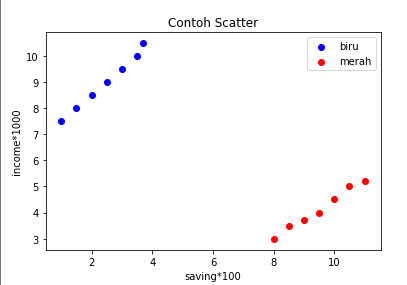
\includegraphics[scale=0.5]{figures/6/Teori/1174025/no3sc.png}
\caption{Contoh Hasil Scatter}
\label{fig:contoh}
\end{figure}
\end{itemize}

\begin{itemize}
	\item Pie\newline
	Chart Pie merupakan grafik yang membentuk sperti kue Pie, dimana cara penggunaannya adalah dengan perintah
	plt.pie seperti pada contoh berikut :
	
	\lstinputlisting[firstline=54, lastline=75]{src/6/Teori/1174025/1174025.py}

\begin{figure}[h]
\centering
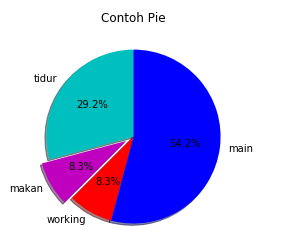
\includegraphics[scale=0.6]{figures/6/Teori/1174025/no3pie.png}
\caption{Contoh Hasil Pie}
\label{fig:contoh Pie}
\end{figure}


\end{itemize}

\subsection{Jelaskan bagaimana cara menggunakan legend dan label serta kaitannya dengan fungsi tersebut}
Legend digunakan untuk menampilkan keterangan tanda pada grafik, label digunakan untuk penamaan tanda tersebut.
berikut adalah syntax untuk menampilkan legend dan penamaan label.

\lstinputlisting[firstline=46, lastline=52]{src/6/Teori/1174025/1174025.py}

\begin{figure}[h]
\centering
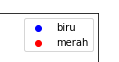
\includegraphics[scale=1]{figures/6/Teori/1174025/no4lg.png}
\caption{Contoh Hasil Legend dan Label}
\label{fig:contoh Legend}
\end{figure}

\subsection{Jelaskan apa fungsi dari subplot di matplotlib, dan bagaimana cara kerja dari fungsi subplot, sertakan ilustrasi dan gambar sendiri dan apa parameternya jika ingin menggambar plot dengan 9 subplot di dalamnya}
Subplot Merupakan Plot didalam dimana Plot ini biasanya berukuran kecil sehingga dapat memuat 2 atau lebih plot dalam 1 paket Plot.\newline
Jika ingin membuat 9 subplot maka buat perintah plt.subplot dengan parameter angka awal 3 angka kedua 3 dan angka ketiga 1, artinya angka awal adalah batas jumlah plot secara vertical, angka kedua adalah batas plot secara horizontal, dan angka ketiga adalah urutan plot nya.
Berikut ini adalah Ilustrasi subplot.

\lstinputlisting[firstline=77, lastline=110]{src/6/Teori/1174025/1174025.py}

\begin{figure}[h]
\centering
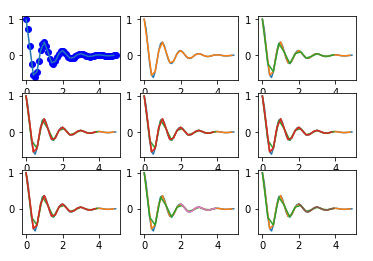
\includegraphics[scale=0.7]{figures/6/Teori/1174025/subplot.png}
\caption{Contoh 9 Subplot}
\label{fig:contoh subplot}
\end{figure}

\subsection{ Sebutkan semua parameter color yang bisa digunakan (contoh: m,c,r,k,... dkk)}
\begin{enumerate}
	\item Parameter yang dapat digunakan adalah CMYK :
\end{enumerate}
 
\begin{itemize}
	\item C = cyan
	\item M = magenta
	\item Y = yellow
	\item K = key
\end{itemize}

\begin{enumerate}
	\item Parameter yang kedua adalah RGB, selain menggunakan RGB nya kita juga dapat menggunakan kode warna dari RGB.
\end{enumerate}

\begin{itemize}
	\item R = red
	\item G = green
	\item B = blue
\end{itemize}

\subsection{Jelaskan bagaimana cara kerja dari fungsi hist, sertakan ilustrasi dan gambar sendiri}
Fungsi hist digunakan untuk memanggil Histogram, diamana Histogram dapat menampilkan grafik sesuai kebutuhan contohnya menampilkan grafik bar, akan tetapi histogram ini tidak mengacu pada sumbu X dan Y, artinya sumbu X dan Y jumlah datanya tidak harus sama. biasanya digunakan untuk menghitung jumlah populasi.\newline
	Cara menggunakannya yaitu dengan perintah plt.hist, Berikut adalah Contohnya :

	\lstinputlisting[firstline=29, lastline=35]{src/6/Teori/1174025/1174025.py}

\begin{figure}[h]
\centering
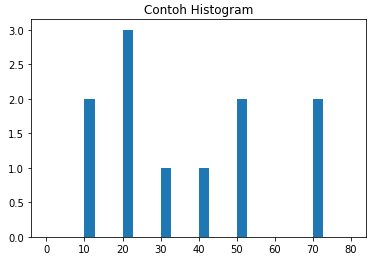
\includegraphics[scale=0.7]{figures/6/Teori/1174025/no3h.png}
\caption{Contoh Hasil Histogram}
\label{fig:contoh}
\end{figure}

\subsection{Jelaskan lebih mendalam tentang parameter dari fungsi pie diantaranya labels, colors, startangle, shadow, explode, autopct}
\begin{itemize}
	\item Labels\newline
	Labels pada Pie adalah untuk menambahkan Keterangan pada Pie diamana labels ini biasanya adalah Variabel yang dialamnya berisi data array
	\item Colors\newline
	Colors pada pie adalah untuk mendefinisikan warna pada setiap potongannya.
	\item Startangle\newline
	Startangle adalah untuk mengatur perputaran potongan Pie nya dimulai dari berapa derajat.
	\item Shadow\newline
	Shadow adalah untuk mengatur ketebalan bayangan pada Pie.
	\item Explode\newline
	Explode ini untuk Mengatur Jarak Pie yang dipotong keluar.
	\item Autopct\newline
	Autopct ini adalah untuk perhitungan persen yang mana kita dapat mengatur berapa angka di belakang koma nya. 
\end{itemize}

\subsection{Plagiarisme}
\begin{figure}[h]
\centering
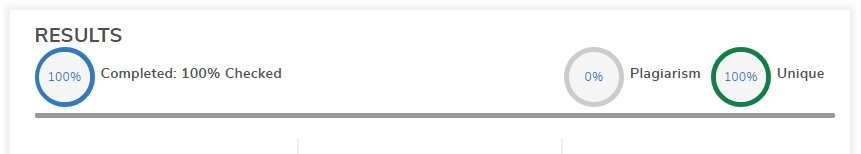
\includegraphics[scale=0.2]{figures/6/Teori/1174025/noplg.png}
\caption{Plagiarisme}
\label{fig:plagiat}
\end{figure}

\section{Evietania}
\subsection{Apa itu fungsi library matplotlib?}
Fungsi dari matplotlip yaitu untuk membuat visualisasi yang kuat dalam menjelaskan suatu data dalam bentuk diagram dan grafik. 
Contoh grafik yang dapat digambarkan menggunakan Matplotlib adalah :
\begin{itemize}
    \item Grafik Biasa 
    \item Chart
    \item Grafik Polar
    \item Dan yang lainnya, berikut adalah contoh dari metlib
\lstinputlisting[firstline=8, lastline=14]{src/6/Teori/1174051/1174051.py}
\end{itemize}

\subsection{Jelaskan langkah-langkah membuat sumbu X dan Y di matplotlib}
Langkah langkah membuat Sumbu X dan Y adalah sebagai berikut :
\begin{itemize}
    \item Buat variabel X dan Y
    \item Masukkan nilai dari setiap variabel
    \lstinputlisting[firstline=9, lastline=10]{src/6/Teori/1174051/1174051.py}
    \item Deklarasikan nama dari sumbu X dan Y yang telah kita buat
    \lstinputlisting[firstline=12, lastline=13]{src/6/Teori/1174051/1174051.py}
\end{itemize}

Setelah kita jalankan, maka beginilah hasil yang diperoleh
\begin{figure}[H]
    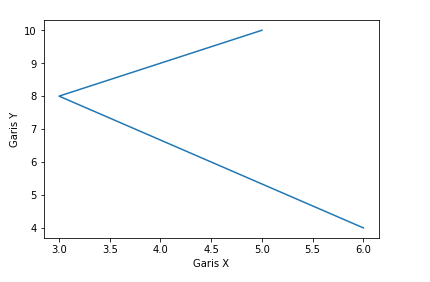
\includegraphics[width=9cm]{figures/6/Teori/1174051/1.png}
    \caption{Hasil dari membuat sumbu X dan Y}
    \centering
\end{figure}

\subsection{Jelaskan bagaimana perbedaan fungsi dan cara pakai untuk berbagai jenis(bar,histogram,scatter,line dll) jenis plot di matplotlib}
\begin{itemize}
    \item Bar\newline
    Bar berfungsi menampilkan grafik secara vertikal biasanya digunakan untuk traffic penjualan.\newline
    Cara menggunakan bar cukup ganti plt.plot menjadi plt.bar

    \lstinputlisting[firstline=19, lastline=26]{src/6/Teori/1174051/1174051.py}

\begin{figure}[h]
\centering
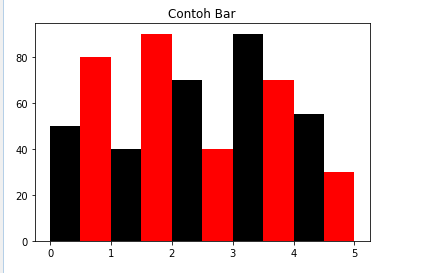
\includegraphics[scale=0.3]{figures/6/Teori/1174051/2.png}
\caption{Hasil Bar}
\label{fig:contoh}
\end{figure}
\end{itemize}

\begin{itemize} 
    \item Histogram\newline
    Histogram dapat menampilkan grafik sesuai kebutuhan contohnya menampilkan grafik bar, akan tetapi histogram ini
    tidak mengacu pada sumbu X dan Y, biasanya digunakanuntuk menghitung jumlah populasi.\newline
    Cara menggunakannya yaitu dengan perintah plt.hist, Berikut adalah Contohnya :

    \lstinputlisting[firstline=29, lastline=35]{src/6/Teori/1174051/1174051.py}

\begin{figure}[h]
\centering
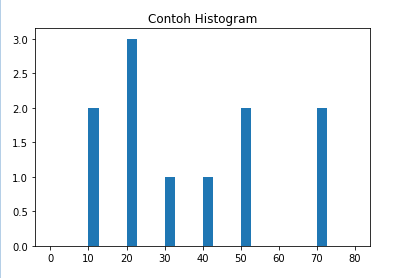
\includegraphics[scale=0.9]{figures/6/Teori/1174051/3.png}
\caption{Hasil Histogram}
\label{fig:contoh}
\end{figure}
\end{itemize}

\begin{itemize}
    \item Line\newline
    Line merupakan Plot grafik yang hanya menggambarkan sebuah garis sesuai kordinat yang kita atur.
    Berikut adalah Contohnya penulisannya :

    \lstinputlisting[firstline=8, lastline=14]{src/6/Teori/1174051/1174051.py}

\begin{figure}[h]
\centering
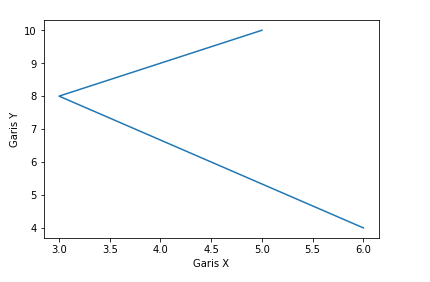
\includegraphics[scale=0.6]{figures/6/Teori/1174051/1.png}
\caption{Plot Line}
\label{fig:contoh}
\end{figure}
\end{itemize}

\begin{itemize} 
    \item Scatter\newline
    Scatter merupakan grafik yang didalamnya dapat berisi 2 data dalam 1 plot.\newline
    Berikut adalah contohnya :

    \lstinputlisting[firstline=38, lastline=52]{src/6/Teori/1174051/1174051.py}

\begin{figure}[h]
\centering
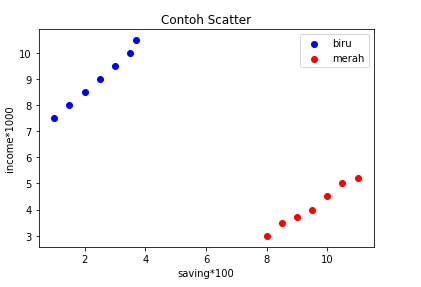
\includegraphics[scale=0.5]{figures/6/Teori/1174051/4.png}
\caption{Hasil Scatter}
\label{fig:contoh}
\end{figure}
\end{itemize}

\begin{itemize}
    \item Pie\newline
    Chart Pie merupakan grafik yang membentuk sperti kue Pie, berikut adalah contohnya:
    
    \lstinputlisting[firstline=55, lastline=75]{src/6/Teori/1174051/1174051.py}

\begin{figure}[h]
\centering
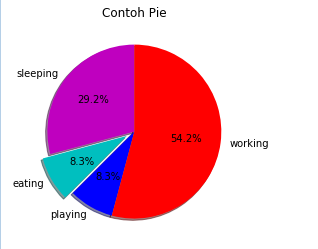
\includegraphics[scale=0.6]{figures/6/Teori/1174051/5.png}
\caption{Hasil Pie}
\label{fig:contoh Pie}
\end{figure}


\end{itemize}

\subsection{Jelaskan bagaimana cara menggunakan legend dan label serta kaitannya dengan fungsi tersebut}
Fungsi legend digunakan untuk menjelaskan makna dari objek berupa titik atau garis di dalam diagram.
berikut adalah contohnya 
\lstinputlisting[caption = fungsi untuk membuat legend., firstline=46, lastline=47]{src/6/Teori/1174051/1174051.py}
contoh legend :
\begin{figure}[H]
    
\includegraphics[width=9cm]{figures/6/Teori/1174051/6.png}
    \caption{contoh legend}
    \centering
\end{figure}

\subsection{Jelaskan apa fungsi dari subplot di matplotlib, dan bagaimana cara kerja dari fungsi subplot, sertakan ilustrasi dan gambar sendiri dan apa parameternya jika ingin menggambar plot dengan 9 subplot di dalamnya}
Subplot berfungsi untuk menggabungkan beberapa plot kedalam satu figure
cara kerjanya adalah sebagai berikut
\lstinputlisting[firstline=78, lastline=110]{src/6/Teori/1174051/1174051.py}

\begin{figure}[h]
\centering
\includegraphics[scale=0.7]{figures/6/Teori/1174051/subplot.png}
\caption{Contoh Subplot}
\label{fig:contoh subplot}
\end{figure}

\subsection{Sebutkan semua parameter color yang bisa digunakan}
Parameter color yang bisa digunakan antara lain RGB dan CMYK
\begin{itemize}
    \item C (Cyan) adalah biru muda
    \item M (Magenta) adalah merah muda
    \item Y (Yellow) adalah kuning
    \item K (Key) adalah hitam
    \item R (Red) adalah merah
    \item G (Green) adalah Hijau
    \item B (Blue) adalah Biru
    
\end{itemize}

\subsection{Jelaskan bagaimana cara kerja dari fungsi hist, sertakan ilustrasi dan gambar sendiri}
cara kerja dari fungsi histogram adalah sebagai berikut :
\lstinputlisting[firstline=29, lastline=35]{src/6/Teori/1174051/1174051.py}

\begin{figure}[h]
\centering
\includegraphics[scale=0.7]{figures/6/Teori/1174051/3.png}
\caption{Contoh Hasil Histogram}
\label{fig:contoh}
\end{figure}

\subsection{Jelaskan lebih mendalam tentang parameter dari fungsi pie diantaranya labels, colors, startangle, shadow, explode, autopct}
\begin{itemize}
    \item Labels = berfungsi untuk menampilkan tulisan pada diagram pie
    \item Colors = berfungsi untuk menentukan warna pada tiap bagian pada diagram pie
    \item Startangle = berfungsi untuk menentukan sudut pertama pada diagram pie
    \item Shadow = berfungsi untuk menampilkan efek timbul pada diagram pie
    \item Explode = berfungsi untuk menunjukkan jarak pisah dari diagram pie.
    \item Autopct = berfungsi umtuk menampilkan jumlah angka dibelakang koma pada bilangan pecahan
\end{itemize}

\subsection{Pengecekan Plagiarisme Teori}
\begin{figure}[H]
    \includegraphics[width=9cm]{figures/6/Teori/1174051/plagiat.png}
    \centering
\end{figure}



%%%%%%%%%%%%%%%%%%%%%%%%%%%%%%%%%%%%%%%%%%%%%%%%%%%%%%%
\section{Oniwaldus Bere Mali}
\subsection{1. Apa itu fungsi library matplotlib?}
Library Matplotlib berfungsi untuk membuat visualisasi yang kuat dalam menjelaskan suatu data dalam bentuk diagram dan grafik. 
Contoh grafik yang dapat digambarkan menggunakan Matplotlib adalah :
\begin{itemize}
\item Grafik Biasa 
\item Grafik Polar
\item Chart
\item Dan yang lainnya
\end{itemize}

\subsection{2. Jelaskan langkah-langkah membuat sumbu X dan Y di matplotlib}
Langkah langkah yang perluh dibuat dalam Sumbu X dan Y adalah sebagai berikut :
\begin{itemize}
\item Buat variabel x dan Y
\item Masukkan nilai dari setiap variabel
\lstinputlisting[firstline=12, lastline=13]{src/6/Teori/1174005/1174005.py}
\item Deklarasikan nama dari sumbu x dan y 
\lstinputlisting[firstline=16, lastline=17]{src/6/Teori/1174005/1174005.py}
\end{itemize}

Setelah dibuat, begini lah hasilnya
\begin{figure}[H]
\includegraphics[width=9cm]{figures/6/Teori/1174005/1.png}
\caption{Hasil membuat sumbu x dan y}
\centering
\end{figure}

\subsection{3.Jelaskan bagaimana perbedaan fungsi dan cara pakai untuk berbagai jenis(bar,histogram,scatter,line dll) jenis plot di matplotlib}
Perbedaan fungsi dapat dilihat sebagai berikut :
\begin{itemize}
\item Graph\linebreak
Fungsi graph digunakan untuk membuat visualisasi berupa grafik.
cara pakainya adalah sebagai berikut :
\lstinputlisting[caption = fungsi untuk membuat graph., firstline=10, lastline=18]{src/6/Teori/1174005/1174005.py}
hasilnya adalah sebagai berikut:
\begin{figure}[H]
\includegraphics[width=9cm]{figures/6/Teori/1174005/3graph.png}
\caption{Hasil graph}
\centering
\end{figure}

\item Bar\linebreak 
Fungsi Bar digunakan untuk membuat visualisasi berupa diagram batang yang berhimpit.
Cara Pakainya adalah sebagai berikut :
\lstinputlisting[caption = fungsi untuk membuat bar., firstline=22, lastline=32]{src/6/Teori/1174005/1174005.py}
hasilnya adalah sebagai berikut:
\begin{figure}[H]
\includegraphics[width=9cm]{figures/6/Teori/1174005/3bar.png}
\caption{Hasil bar}
\centering
\end{figure}

\item Histogram\linebreak
Fungsi Histogram digunakan untuk membuat visualisasi berupa diagram batang yang tidak berhimpit.
Cara Pakainya adalah sebagai berikut :
\lstinputlisting[caption = fungsi untuk membuat histogram., firstline=35, lastline=42]{src/6/Teori/1174005/1174005.py}
hasilnya adalah sebagai berikut:
\begin{figure}[H]
\includegraphics[width=9cm]{figures/6/Teori/1174005/3histogram.png}
\caption{Hasil histogram}
\centering
\end{figure}

\item Scatter\linebreak
Fungsi Scatter digunakan untuk membuat visualisasi berupa titik titik.
Cara Pakainya adalah sebagai berikut :
\lstinputlisting[caption = fungsi untuk membuat scatter., firstline=45, lastline=58]{src/6/Teori/1174005/1174005.py}
hasilnya adalah sebagai berikut:
\begin{figure}[H]
\includegraphics[width=9cm]{figures/6/Teori/1174005/3scatter.png}
\caption{Hasil scatter}
\centering
\end{figure}

\item Area plot\linebreak
Fungsi Area plot digunakan untuk membuat visualisasi berupa area.
Cara Pakainya adalah sebagai berikut :
\lstinputlisting[caption = fungsi untuk membuat area plot., firstline=61, lastline=80]{src/6/Teori/1174005/1174005.py}
hasilnya adalah sebagai berikut:
\begin{figure}[H]
\includegraphics[width=9cm]{figures/6/Teori/1174005/3areaplot.png}
\caption{Hasil area plot}
\centering
\end{figure}

\item Pie\linebreak
Fungsi Pie digunakan untuk membuat visualisasi berupa diagram lingkaran.
Cara Pakainya adalah sebagai berikut :
\lstinputlisting[caption = fungsi untuk membuat pie., firstline=83, lastline=104]{src/6/Teori/1174005/1174005.py}
hasilnya adalah sebagai berikut:
\begin{figure}[H]
\includegraphics[width=9cm]{figures/6/Teori/1174005/3pie.png}
\caption{Hasil pie}
\centering
\end{figure}
\end{itemize}

\subsection{4.Jelaskan bagaimana cara menggunakan legend dan label serta kaitannya dengan fungsi tersebut}
Fungsi legend digunakan untuk menjelaskan makna dari objek berupa titik atau garis di dalam diagram.
cara menggunakan legend adalah 
\lstinputlisting[caption = fungsi untuk membuat legend., firstline=24, lastline=28]{src/6/Teori/1174005/1174005.py}
contoh legend :
\begin{figure}[H]
\includegraphics[width=9cm]{figures/6/Teori/1174005/4legend.png}
\caption{contoh legend}
\centering
\end{figure}

\subsection{5.Jelaskan apa fungsi dari subplot di matplotlib, dan bagaimana cara kerja dari fungsi subplot, sertakan ilustrasi dan gambar sendiri dan apa parameternya jika ingin menggambar plot dengan 9 subplot di dalamnya}
Subplot berfungsi untuk menggabungkan beberapa plot kedalam satu figure
cara kerjanya adalah sebagai berikut
\lstinputlisting[caption = cara kerja subplot., firstline=108, lastline=134]{src/6/Teori/1174005/1174005.py}
Parameter yang digunakan ketika ingin membuat 9 subplot terdiri dari (331) sampai (339). karena posisi subplot dilihat dengan melihat tinggi,lebar,urutan
hasil dari subplot adalah
\begin{figure}[H]
\includegraphics[width=9cm]{figures/6/Teori/1174005/5subplot.png}
\caption{hasil subplot}
\centering
\end{figure}

\subsection{6.Sebutkan semua parameter color yang bisa digunakan}
Parameter color yang bisa digunakan antara lain RGB dan CMYK
\begin{itemize}
\item C (Cyan) adalah biru muda
\item M (Magenta) adalah merah muda
\item Y (Yellow) adalah kuning
\item K (Key) adalah hitam
\item R (Red) adalah merah
\item G (Green) adalah Hijau
\item B (Blue) adalah Biru
\end{itemize}

\subsection{7.Jelaskan bagaimana cara kerja dari fungsi hist, sertakan ilustrasi dan gambar sendiri}
cara kerja dari fungsi histogram adalah sebagai berikut :
\lstinputlisting[caption = cara kerja histogram., firstline=137, lastline=144]{src/6/Teori/1174005/1174005.py}
hasilnya adalah
\begin{figure}[H]
\includegraphics[width=9cm]{figures/6/Teori/1174005/7his.png}
\caption{histogram}
\centering
\end{figure}

\subsection{8.Jelaskan lebih mendalam tentang parameter dari fungsi pie diantaranya labels, colors, startangle, shadow, explode, autopct}
\begin{itemize}
\item Labels = berfungsi untuk menampilkan tulisan pada diagram pie
\item Colors = berfungsi untuk menentukan warna pada tiap bagian pada diagram pie
\item Startangle = berfungsi untuk menentukan sudut pertama pada diagram pie
\item Shadow = berfungsi untuk menampilkan efek timbul pada diagram pie
\item Explode = berfungsi untuk menunjukkan jarak pisah dari diagram pie.
\item Autopct = berfungsi umtuk menampilkan jumlah angka dibelakang koma pada bilangan pecahan
\end{itemize}

\subsection{Pengecekan Plagiarisme Teori}
\begin{figure}[H]
\includegraphics[width=9cm]{figures/6/Teori/1174005/Plagiat.png}
\centering
\end{figure}
